\section{Qubits}
As defined earlier, qubits are quantum systems whose state space has cardinality of two. The standard orthonormal basis of qubits are denoted by $|0\rangle$ and $|1\rangle$(also known as \textit{standard computational basis}. So, any value of a qubit can be expressed as
\begin{equation}
|\psi\rangle = \alpha | 0\rangle + \beta |1 \rangle
\end{equation}
where $\alpha$ and $\beta$ are complex numbers such that $\| |\psi \rangle \| =1$. As mentioned in the postulates of quantum mechanics, we can't directly measure $\alpha$ and $\beta$. So,  the algorithms must bee designed in such a way that it does not require explicit knowledge of $\alpha$ and $\beta$. So, although we may do various things to manipulate $\alpha$ and $\beta$ but it is very difficult to retrieve that result from the result. This inability restricts us from using the immense power we get from having infinite states(as compared to the two states in the classical bits).
\subsection{Bloch Sphere}
From the normal condition, we get $\alpha^2  + \beta^2 =1$. So, we may re-write $\alpha = e^{i\gamma} \cos{\frac{\theta}{2}} $ and $\beta = e^{i(\gamma+\phi)} \sin{\frac{\theta}{2}} $ . So, we get
\begin{equation}
|\psi \rangle = e^{i\gamma} \left( \cos{\frac{\theta}{2}} |0\rangle + e^{i\phi} \sin{\frac{\theta}{2}} |1\rangle \right)
\end{equation}The overall phase $e^{i\gamma}$ has no effect as it has no \textit{observable effects} and hence can be neglected. So,
\begin{equation}
|\psi \rangle = \cos{\frac{\theta}{2}} |0\rangle + e^{i\phi} \sin{\frac{\theta}{2}} |1\rangle 
\end{equation}
The numbers $\theta$ and $\phi$ define a point on a unit sphere where $\theta$ is the angle from z-axis and $\phi$ is the angle projection of point makes with the x-axis. 
\begin{figure}[t]
\centering
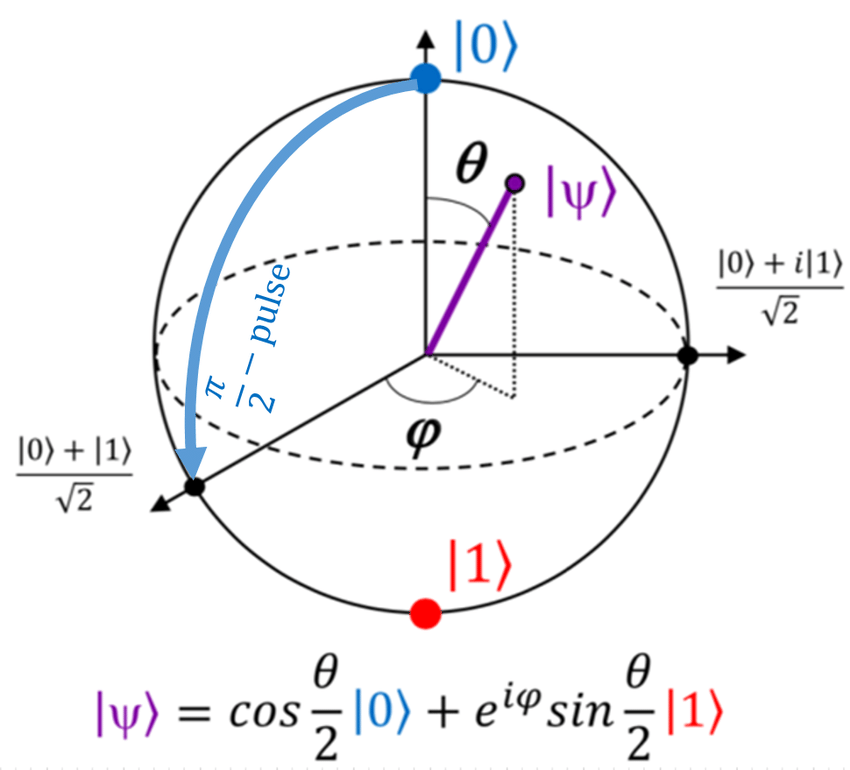
\includegraphics[width=0.5\textwidth]{images/blochsphere.png}\par
\label{blochsphere}
\caption{Bloch sphere representation of a qubit}
\end{figure}
It turns out that any operation on a qubit can be represented by a rotation in the bloch sphere notation. 
